\section{Bakti Qilan Mufid (1174083)}
\subsection{Instalasi Map Server}
\begin{enumerate}
	\item  Download installer Map Server di ms4w.com . Pilih yang .exe.
	\hfill\break
	\begin{figure}[H]
		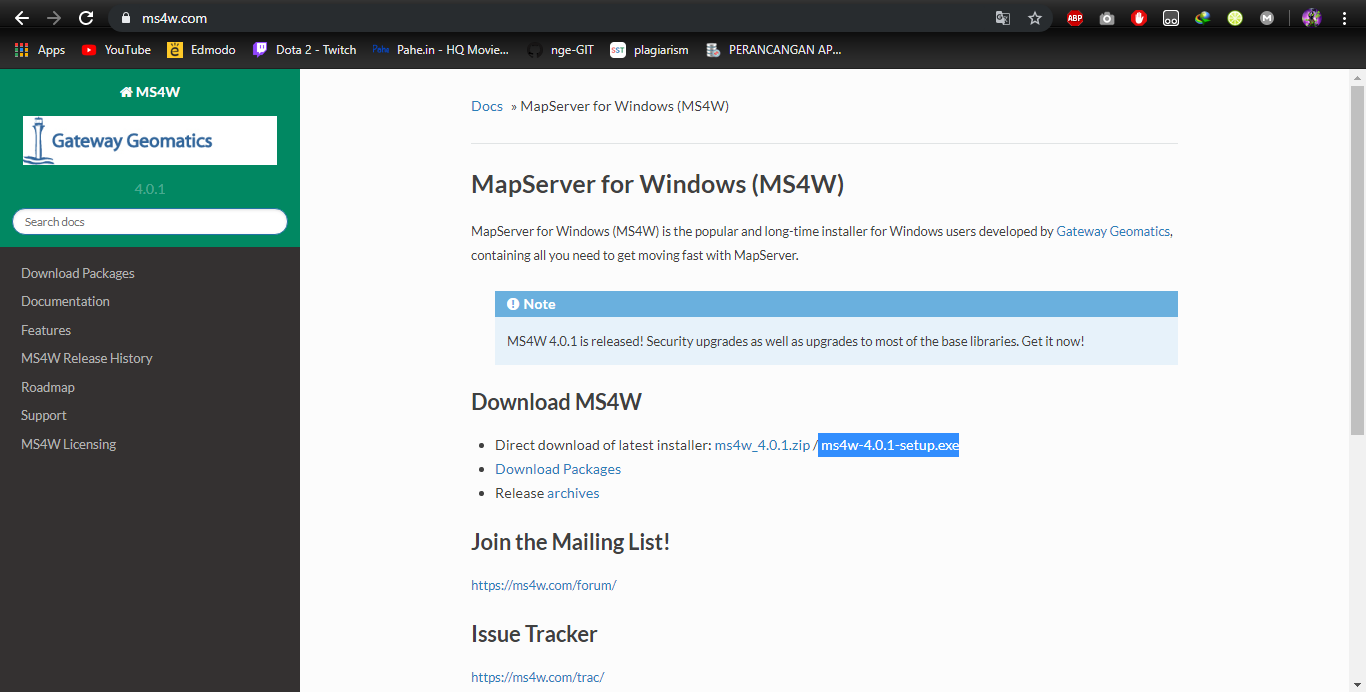
\includegraphics[width=8cm]{figures/Tugas4/1174083/pic1.png}
		\centering
		\caption{Download installer Map Server.}
	\end{figure}
	\item  Setelah selesai di download, klik dua kali pada installer.
	\hfill\break
	\begin{figure}[H]
		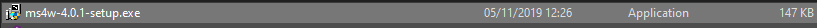
\includegraphics[width=8cm]{figures/Tugas4/1174083/pic2.png}
		\centering
		\caption{Klik dua kali pada installer.}
	\end{figure}
	\item  Kemudian klik "I Agree".
	\hfill\break
	\begin{figure}[H]
		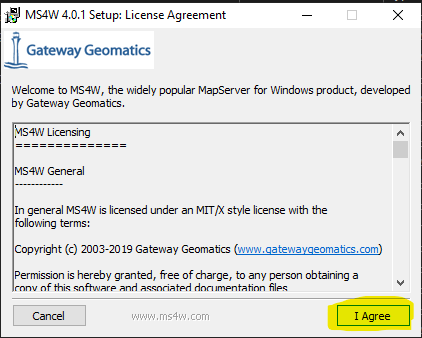
\includegraphics[width=8cm]{figures/Tugas4/1174083/pic3.png}
		\centering
		\caption{Klik "I Agree".}
	\end{figure}
	\item  Pilih tipe instalasinya yang "Full". Kemudian klik Next.
	\hfill\break
	\begin{figure}[H]
		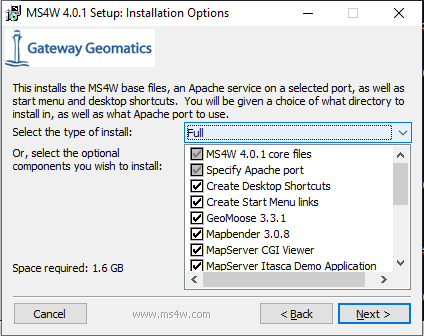
\includegraphics[width=8cm]{figures/Tugas4/1174083/pic4.png}
		\centering
		\caption{Tipe instalasi "Full".}
	\end{figure}
	\item  Pilih direktori instalasinya. Kemudian klik Next.
	\hfill\break
	\begin{figure}[H]
		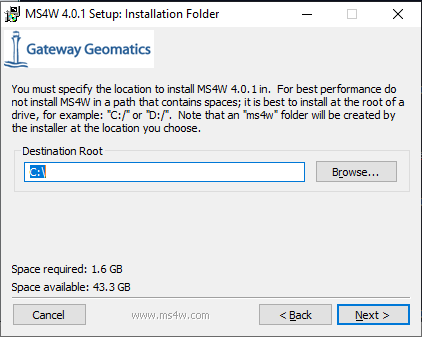
\includegraphics[width=8cm]{figures/Tugas4/1174083/pic5.png}
		\centering
		\caption{Pilih direktori instalasi}
	\end{figure}
	\item  Isi port Apache yang akan dipakai. Kemudian klik Next.
	\hfill\break
	\begin{figure}[H]
		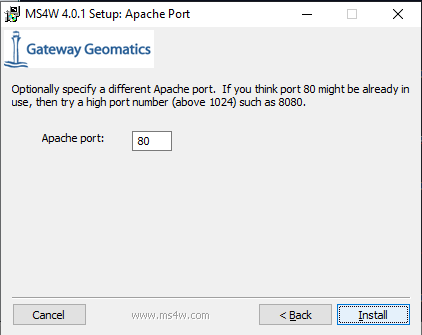
\includegraphics[width=8cm]{figures/Tugas4/1174083/pic6.png}
		\centering
		\caption{Isi port Apache.}
	\end{figure}
	\item  Tunggu hingga proses instalasi selesai.
	\hfill\break
	\begin{figure}[H]
		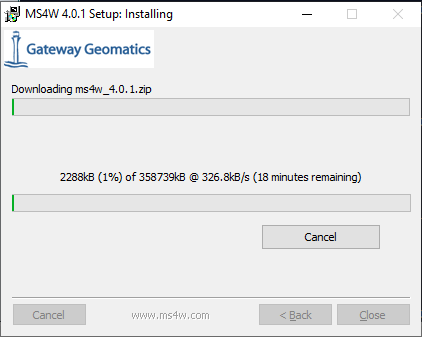
\includegraphics[width=8cm]{figures/Tugas4/1174083/pic7.png}
		\centering
		\caption{Proses instalasi.}
	\end{figure}
	\item  Klik Close.
	\hfill\break
	\begin{figure}[H]
		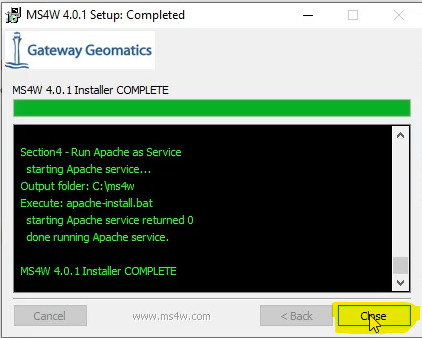
\includegraphics[width=8cm]{figures/Tugas4/1174083/pic8.png}
		\centering
		\caption{Akhir proses instalasi.}
	\end{figure}
\end{enumerate}


\subsection{Link Youtube}
https://youtu.be/oePUu9IP6FA


\subsection{Instalasi Map Proxy}
\begin{enumerate}
	\item  Ketik peritah berikut di CMD.
	\hfill\break
	\begin{figure}[H]
		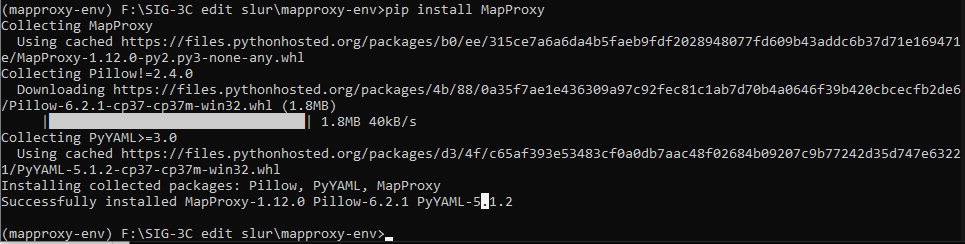
\includegraphics[width=8cm]{figures/Tugas4/1174083/pic10.png}
		\centering
		\caption{Install Map Proxy}
	\end{figure}
	\item  Ketik peritah berikut di CMD.
	\hfill\break
	\begin{figure}[H]
		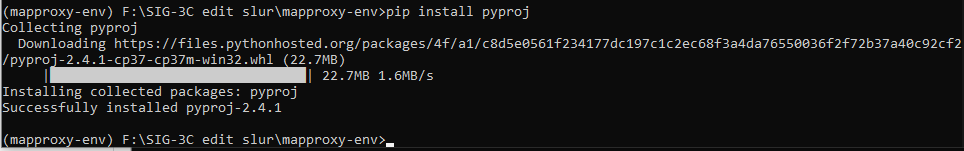
\includegraphics[width=8cm]{figures/Tugas4/1174083/pic11.png}
		\centering
		\caption{Install pyproj}
	\end{figure}
\end{enumerate}
\subsection{Link Youtube}
https://youtu.be/oePUu9IP6FA

\subsection{Membuka map menggunakan MapProxy}
\begin{enumerate}
  \item Download / clone git dari https://github.com/awangga/gede	
  \item Pada folder gede-master buat folder bernama tmp
  \hfill\break
  \begin{figure}[H]
  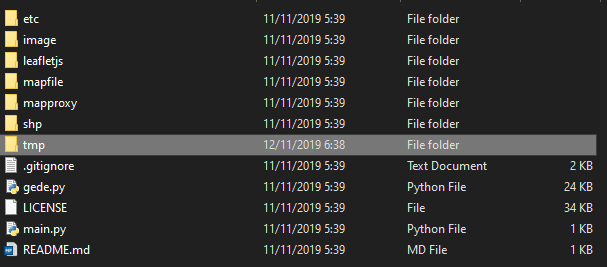
\includegraphics[width=4cm]{figures/Tugas4/1174083/pic13.png}
  \centering
  \caption{Buat folder tmp}
  \end{figure}

  \item Setelah itu buka folder mapproxy lalu edit file agm.yaml
  \hfill\break
  \begin{figure}[H]
  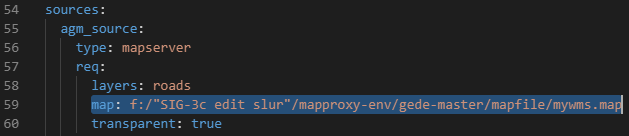
\includegraphics[width=4cm]{figures/Tugas4/1174083/pic14.png}
  \centering
  \caption{File agm.yaml}
  \end{figure}

  \item Edit pada bagian sources lalu ada map, masukkan pathnya sesuai dengan dimana anda menyimpan file gede yang anda clone contohnya saya ada pada /gede-master/mapfile/mywms.map
  \item Lalu dibawahnya pada bagian binary masukkan lokasi instalasi ms4w anda, lalu tambahkan /Apache/cgi-bin/mapserv.exe, yang saya setelah diedit menjadi C:/ms4w/Apache/cgi-bin/mapserv.exe dan pada bagian working-dir masukkan path folder yang telah kita buat tadi, yang saya /gede-master/tmp
  \hfill\break
  \begin{figure}[H]
  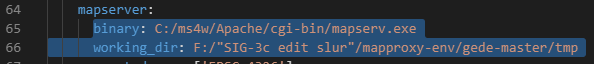
\includegraphics[width=4cm]{figures/Tugas4/1174083/pic15.png}
  \centering
  \caption{Edit lokasi mymap.map}
  \end{figure}

  \item Setelah itu buka aplikasi MS4W-Shell
  \hfill\break
  \begin{figure}[H]
  \includegraphics[width=4cm]{figures/Tugas4/1174083/pic16.png}
  \centering
  \caption{Aplikasi MS4W-Shell}
  \end{figure}

  \item Setelah itu buka lokasi folder gede kita yang tadi telah di clone
  \hfill\break
  \begin{figure}[H]
  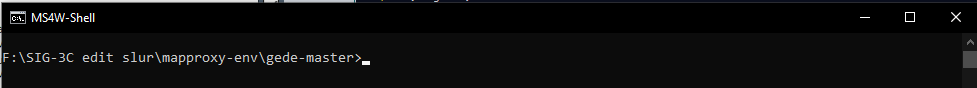
\includegraphics[width=4cm]{figures/Tugas4/1174083/pic17.png}
  \centering
  \caption{Buka Folder gede}
  \end{figure}

  \item Setelah itu buka folder mapproxy yang ada pada folder gede
  \hfill\break
  \begin{figure}[H]
  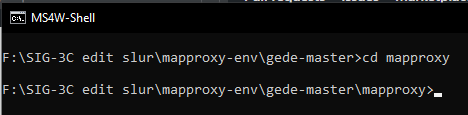
\includegraphics[width=4cm]{figures/Tugas4/1174083/pic18.png}
  \centering
  \caption{Buka Folder mapproxy}
  \end{figure}

  \item setelah dibuka ketikkan "mapproxy-util serve-develop ./agm.yaml" pada ms4w-Shell untuk membuka aplikasi mapproxy
  \hfill\break
  \begin{figure}[H]
  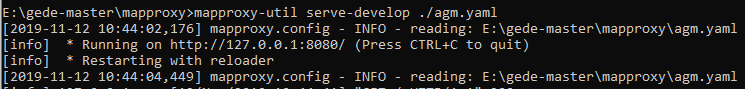
\includegraphics[width=4cm]{figures/Tugas4/1174083/pic19.png}
  \centering
  \caption{Buka aplikasi mapproxy}
  \end{figure}
  
  \item Buka browser lalu ketikkan 127.0.0.1:8080
  \hfill\break
  \begin{figure}[H]
  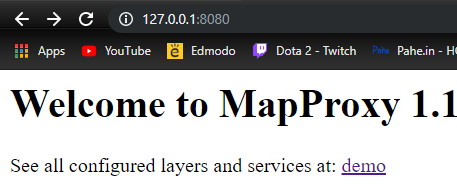
\includegraphics[width=4cm]{figures/Tugas4/1174083/pic20.png}
  \centering
  \caption{Buka mapproxy pada browser}
  \end{figure}

  \item lalu klik demo untuk melihat map
  \item lalu klik png pada agm, maka mapproxy akan menampilkan map
  \hfill\break
  \begin{figure}[H]
  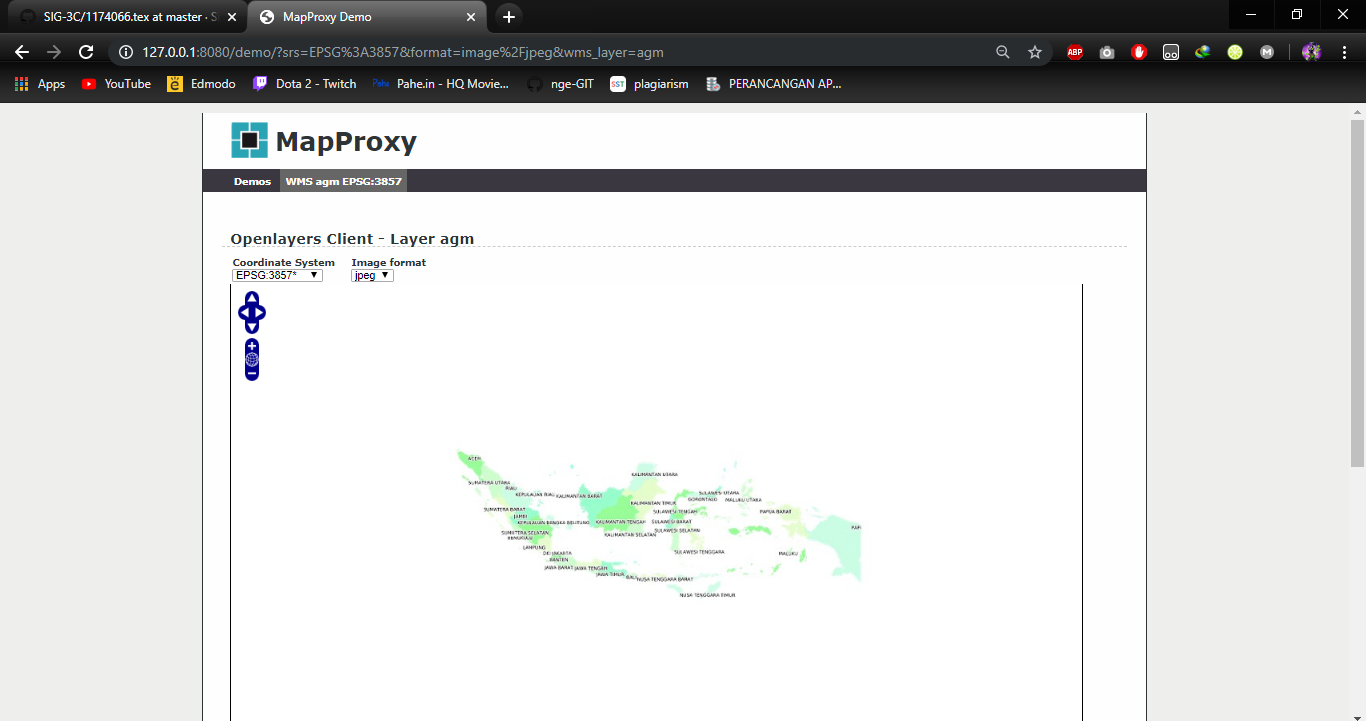
\includegraphics[width=4cm]{figures/Tugas4/1174083/pic22.png}
  \centering
  \caption{MapProxy menampilkan map}
  \end{figure}

\end{enumerate}

\subsection{Link Youtube MapProxy dan Menjalankannya}
https://youtu.be/MKw4QSOa20M